% ============================================================
%  Computational Complexity section --- ModSim paper.
%  Placement: after System Architecture (sec:architecture).
%  Target: IEEE conference template (IEEEtran, two-column).
%
%  >>> PREAMBLE REQUIREMENTS (add once, if not already present):
%     \usepackage{graphicx}
%     \usepackage{booktabs}   % already loaded for the related-work table
%     \usepackage{amsmath}
%
%  Figure: fig_complexity.pdf, produced by
%     python scripts/complexity/bench_complexity.py --out results/complexity
%     python scripts/complexity/plot_complexity.py results/complexity docs/paper/fig_complexity.pdf
%  >>> Numbers below were measured on a 2-core x86-64 Linux VM (Python 3.13,
%      MuJoCo 3.11). Re-run on the machine reported in the paper and update the
%      per-unit costs in Table~\ref{tab:complexity} and the text before submission.
% ============================================================

\section{Computational Complexity}
\label{sec:complexity}

A modular-robot layer is only useful if it does not become the bottleneck as
the module count grows. We therefore bound the cost of every stage ModSim adds
to a physics step, and measure each bound in isolation.
We write $N$ for modules, $C$ for connector instances ($C=cN$ for a pack with
$c$ connectors per module; $c=14$ for M-Blocks), $F\le C$ for free
(unengaged) connectors, $E$ for active connections, $K$ for connector pairs
inside the broad-phase radius, $A$ for the size of the assembly an event touches,
and $P$ for the pre-allocated constraint-pool capacity ($P=\Theta(N)$ in all our
scenes).

\noindent\textbf{Per tick.}\ One \texttt{step} runs the engine, takes a
snapshot, ingests it into \texttt{WorldState}, checks connection overloads, and
optionally runs a passive docking pass (Table~\ref{tab:complexity}). The
snapshot is a single vectorised copy of the needed engine arrays through index
arrays fixed at load time; poses, twists, joint states, and connector frames are
materialised in $O(1)$ each, only when read. Ingest is $O(N+C)$: it adopts the
snapshot per module and resets per-step connector detection flags, while module
root states and connector frames resolve lazily against the current sample.
Overload checking is $O(E)$. The docking pass resolves each free connector's
frame, inserts it into a uniform spatial hash whose cell size is the largest
acceptance radius, and evaluates the $K$ surviving pairs in sorted order, for
$O(F + K\log K)$. The hash is linear rather than quadratic because rigid modules
cannot interpenetrate, so only a geometry-dependent constant number of
connectors can lie within any cell's neighbourhood; the same argument bounds
$K=O(F)$.

\noindent\textbf{Per event.}\ \texttt{WorldState} maintains module adjacency
incrementally, so a dock commit merges two assemblies in $O(A_1+A_2)$ and an
undock splits one by a breadth-first walk of the affected assembly alone, in
$O(A)$; neither touches the rest of the world. On the backend side, MuJoCo
fixes the constraint set at compile time~\cite{todorov2012mujoco}, so a dock or
undock activates or deactivates a pre-allocated weld slot ($O(P)$ slot search,
$O(P\log P)$ contact-exclusion update) and refreshes the position and velocity
kinematics that snapshots read ($T_{\mathrm{kin}}(N)$: \texttt{mj\_kinematics},
\texttt{mj\_comPos}, \texttt{mj\_comVel}). A full \texttt{mj\_forward} is not
needed: its collision and constraint results are recomputed by the next step,
and the solver warm start is written only by \texttt{mj\_step}, so the cheaper
refresh leaves every trajectory bit-identical.

\begin{table}[t]
  \centering
  \caption{Cost of each ModSim stage. Bounds follow from the implementation;
    per-unit costs are least-squares slopes of the sweeps in
    Fig.~\ref{fig:complexity} (M-Blocks for per-tick rows; generic cubes for
    connections and events). Backend rows add to the core rows.}
  \label{tab:complexity}
  \footnotesize
  \setlength{\tabcolsep}{3pt}
  \begin{tabular}{@{}lll@{}}
    \toprule
    Stage & Bound & Measured \\
    \midrule
    \multicolumn{3}{@{}l}{\emph{Every tick}} \\
    \quad MuJoCo step & $T_{\mathrm{phys}}(N)$ & 10.9\,$\mu$s/module \\
    \quad Snapshot & $O(N{+}C{+}E\log E)$ & 1.1\,$\mu$s/module \\
    \quad Ingest & $O(N{+}C)$ & 5.0\,$\mu$s/module \\
    \quad Overload check & $O(E)$ & 2.1\,$\mu$s/connection \\
    \quad Passive docking & $O(F{+}K\log K)$ & 27\,$\mu$s/free connector \\
    & & ${+}$37\,$\mu$s/candidate pair \\
    \midrule
    \multicolumn{3}{@{}l}{\emph{Per dock or undock}} \\
    \quad Dock, core & $O(A_1{+}A_2)$ & 0.033\,ms, flat in $N$ \\
    \quad Undock, core & $O(A)$ & 0.022\,ms, flat in $N$ \\
    \quad Backend, MuJoCo & $O(P\log P){+}T_{\mathrm{kin}}(N)$ & 0.2--0.6\,$\mu$s/module \\
    \bottomrule
  \end{tabular}
\end{table}

\begin{figure}[t]
  \centering
  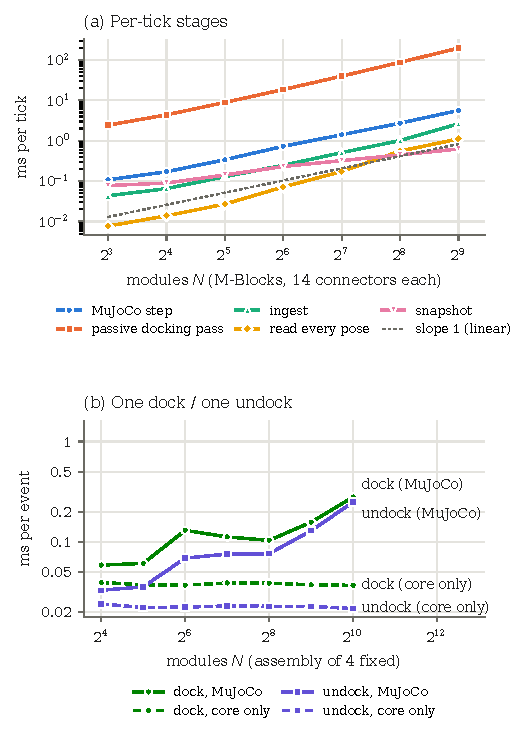
\includegraphics[width=\columnwidth]{fig_complexity.pdf}
  \caption{Measured stage costs on log--log axes. (a) Per tick, against the
    number of free-standing M-Blocks on the MuJoCo backend; the dotted line has
    slope one. Every stage is linear in $N$; the passive docking pass is the
    largest term. (b) One dock and one undock in a fixed four-module assembly,
    against total module count, on the core-only mock backend and on MuJoCo.}
  \label{fig:complexity}
\end{figure}

\noindent\textbf{Measurements.}\ Fig.~\ref{fig:complexity} and
Table~\ref{tab:complexity} report each stage while one quantity varies and the
others stay fixed. Every per-tick stage is linear in $N$ (log--log slopes
$1.00$--$1.12$ for the physics step, ingest, and docking pass; the snapshot is
sublinear over this range because its fixed cost still dominates at $N\le 512$).
Detection is linear in $K$ at fixed $N$ ($R^2=1.00$), confirming that the
broad phase, not pair evaluation, sets its floor. Core dock and undock costs are
flat in $N$ (0.037\,ms and 0.022\,ms from 16 to 1024 modules); undock grows
only with the size of the assembly it splits.

Two consequences matter in practice. First, a passive docking pass costs more
than the physics step it accompanies---195\,ms against 5.6\,ms for 512 M-Blocks
(7168 connectors)---because each free connector's frame is resolved in
interpreted code. ModSim therefore lets scenarios disable passive capture
during transit and request docks explicitly at landing, which the M-Blocks
demonstrations do; capture is then evaluated only while a module is landing.
Second, the only per-event work that still scales with the whole world is
MuJoCo's kinematics refresh and contact-exclusion update, because the engine
offers no per-island update. Their constant is small: 0.24\,ms per event at
384 M-Blocks against 3.3\,ms for one physics step, whereas the full
\texttt{mj\_forward} this replaces costs as much as the step itself (3.2\,ms).
When the number of independently reconfiguring robots grows with $N$, the event
term still grows as $O(N^2)$ per simulated second, but it stays negligible at
practical scales: our multi-copy benchmark averages $0.0017$ topology changes
per copy per tick ($0.11$ per tick at 64 copies), so events add under 1\% of
the physics cost there, and extrapolating, they would match the physics step
only near 50\,000 modules (about 3500 with a full \texttt{mj\_forward} per
event).

Finally, the lazy snapshot path is what keeps ModSim's own per-tick cost below
the engine's. Building every pose, twist, and connector frame eagerly cost
142\,s of state synchronisation in a 384-module, one-simulated-second run;
the array-backed snapshot with on-demand materialisation reduces this to
7.5\,s while producing bit-identical trajectories across all our regression
scenarios.
